\documentclass[aspectratio=169,11pt,t]{beamer}

% ============================================================
% Theme and typography
% ============================================================

\usetheme{Madrid}
\usecolortheme{default}
\usefonttheme{professionalfonts}

\setbeamertemplate{navigation symbols}{}
\setbeamertemplate{headline}{}

\setbeamertemplate{footline}{%
  \leavevmode\hbox{%
  \begin{beamercolorbox}[wd=.82\paperwidth,ht=2.5ex,dp=1.0ex,leftskip=.8em]{author in head/foot}
    CSCI 6461 --- Computer Systems Architecture
  \end{beamercolorbox}%
  \begin{beamercolorbox}[wd=.18\paperwidth,ht=2.5ex,dp=1.0ex,rightskip=.8em]{date in head/foot}
    \hfill\insertframenumber/\inserttotalframenumber
  \end{beamercolorbox}}
}

\setbeamersize{
  text margin left=0.65cm,
  text margin right=0.65cm
}

\setbeamerfont{frametitle}{size=\Large, series=\bfseries}
\setbeamerfont{block title}{size=\normalsize, series=\bfseries}
\setbeamertemplate{blocks}[rounded][shadow=false]

% Block vertical padding adjustments
\addtobeamertemplate{block begin}{\vspace{0.1em}}{\vspace{0.1em}}
\addtobeamertemplate{block end}{}{\vspace{0.2em}}

% Base list item separation
\setbeamertemplate{itemize/enumerate body begin}{\setlength{\itemsep}{4pt}}
\setbeamertemplate{itemize/enumerate subbody begin}{\setlength{\itemsep}{2pt}}

% ============================================================
% Packages
% ============================================================

\usepackage[T1]{fontenc}
\usepackage{lmodern}
\usepackage{amsmath}
\usepackage{booktabs}
\usepackage{array}
\usepackage{tikz}

\usetikzlibrary{
  arrows.meta,
  positioning,
  shapes.geometric,
  calc
}

% ============================================================
% Colors
% ============================================================

\definecolor{navy}{RGB}{24,43,68}
\definecolor{deepblue}{RGB}{45,88,130}
\definecolor{lightblue}{RGB}{235,242,250}
\definecolor{softgray}{RGB}{245,247,250}
\definecolor{darkgray}{RGB}{25,28,32}
\definecolor{gold}{RGB}{200,145,35}

\setbeamercolor{palette primary}{bg=navy,fg=white}
\setbeamercolor{palette secondary}{bg=deepblue,fg=white}
\setbeamercolor{frametitle}{bg=navy,fg=white}
\setbeamercolor{title}{fg=white}
\setbeamercolor{subtitle}{fg=white}
\setbeamercolor{author}{fg=white}
\setbeamercolor{date}{fg=white}
\setbeamercolor{titlelike}{fg=white}
\setbeamercolor{block title}{bg=deepblue,fg=white}
\setbeamercolor{block body}{bg=lightblue,fg=darkgray}
\setbeamercolor{normal text}{fg=darkgray,bg=white}

% ============================================================
% Formatting shortcuts
% ============================================================

\setlength{\parskip}{0pt}

\newcommand{\key}[1]{\textbf{#1}}
\newcommand{\bits}[1]{\texttt{#1}}
\newcommand{\hex}[1]{\texttt{0x#1}}
\newcommand{\code}[1]{\texttt{#1}}

% Section divider macro
\newcommand{\sectiondivider}[2]{%
\begin{frame}[plain]
\begin{tikzpicture}[remember picture,overlay]
\fill[navy] (current page.south west) rectangle (current page.north east);
\fill[gold] (current page.south west) rectangle ([yshift=.15cm]current page.south east);
\end{tikzpicture}
\vspace*{\fill}
\begin{minipage}{0.85\textwidth}
{\color{gold}\large\bfseries #1\par}
\vspace{0.3cm}
{\color{white}\fontsize{22}{26}\selectfont\bfseries #2\par}
\end{minipage}
\vspace*{\fill}
\end{frame}
}

% ============================================================
% Metadata
% ============================================================

\title[Topic 2]{
  RISC vs. CISC:\\
  Instruction Set Design Principles \& Trade-offs
}

\subtitle{
  ISA boundaries, microarchitectural costs,
  and quantitative trade-offs
}

\author{
  Computer Systems Architecture
}

\date{}

% ============================================================
% Document
% ============================================================

\begin{document}

% ============================================================
% Slide 1: Title Slide
% ============================================================

\begin{frame}[plain]
\begin{tikzpicture}[remember picture,overlay]
\fill[navy] (current page.south west) rectangle (current page.north east);
\fill[gold] (current page.south west) rectangle ([yshift=.15cm]current page.south east);
\end{tikzpicture}

\vspace*{\fill}
\begin{minipage}{0.88\textwidth}
{\color{gold}\normalsize\bfseries CSCI 6461 \;|\; TOPIC 2\par}
\vspace{0.25cm}
{\color{white}\fontsize{24}{28}\selectfont\bfseries
 RISC vs. CISC:\\[0.08cm]
 Instruction Set Design Principles \& Trade-offs
\par}
\vspace{0.35cm}
{\color{white!80}\large
 ISA boundaries, microarchitectural costs,
 and quantitative trade-offs
\par}
\end{minipage}

\vfill
{\color{white}\normalsize Dr. J. Burns\par}
{\color{white!70}\small Computer Systems Architecture --- AArch64 Reference Platform\par}
\vspace*{\fill}
\end{frame}

% ============================================================
% Slide 2: Topics Overview
% ============================================================

\begin{frame}{Topic 2: Module Roadmap}

\begin{enumerate}\setlength{\itemsep}{8pt}
  \item \key{ISA Foundations \& Complexity Distribution}
  \begin{itemize}
    \item The programmer-visible hardware contract and historical constraints.
  \end{itemize}

  \item \key{The CISC Architectural Model}
  \begin{itemize}
    \item Register-memory operations, variable-length encodings, and microarchitectural costs.
  \end{itemize}

  \item \key{The RISC Revolution \& Principles}
  \begin{itemize}
    \item Load/store discipline, fixed 32-bit width, and side-by-side assembly comparison.
  \end{itemize}

  \item \key{Quantitative Performance, Energy \& Modern Convergence}
  \begin{itemize}
    \item Iron Law evaluation, Amdahl's Law, performance-per-watt, and modern $\mu\text{op}$ cracking.
  \end{itemize}
\end{enumerate}

\end{frame}

% ============================================================
% Section 1 Divider
% ============================================================

\sectiondivider{PART 1}{ISA Foundations \& Historical Context}

% ============================================================
% Slide 3
% ============================================================

\begin{frame}{What Is an Instruction Set Architecture?}
\begin{itemize}\setlength{\itemsep}{7pt}
  \item An ISA is the \key{programmer-visible functional specification} of a processor.
  \item Defines instructions, register files, addressing modes, and architectural state.
  \item Sits directly at the hardware/software boundary as a rigid abstraction contract.
  \item \key{Complexity Redistribution:} ISA design redistributes complexity between software (compilers) and hardware (microarchitectures).
\end{itemize}

\vfill
\centering
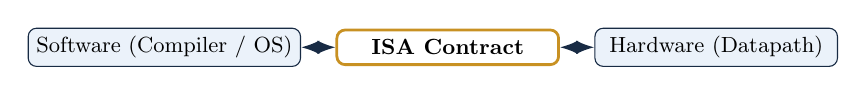
\begin{tikzpicture}[scale=0.88, every node/.style={transform shape}]
  \node[draw=navy, fill=lightblue, rounded corners=3pt, font=\small, minimum width=3.5cm, minimum height=0.5cm] (sw) {Software (Compiler / OS)};
  \node[draw=gold, fill=white, line width=1pt, rounded corners=3pt, font=\small\bfseries, right=0.5cm of sw, minimum width=3.2cm, minimum height=0.5cm] (isa) {ISA Contract};
  \node[draw=navy, fill=lightblue, rounded corners=3pt, font=\small, right=0.5cm of isa, minimum width=3.5cm, minimum height=0.5cm] (hw) {Hardware (Datapath)};
  \draw[{Latex}-{Latex}, thick, navy] (sw) -- (isa);
  \draw[{Latex}-{Latex}, thick, navy] (isa) -- (hw);
\end{tikzpicture}

\vfill
\small
A well-designed ISA survives decades of microarchitectural overhauls by maintaining this strict software contract while hardware implementation evolves underneath it.
\end{frame}

% ============================================================
% Slide 4
% ============================================================

\begin{frame}{Historical Constraints Shaped Early ISAs (CISC Era)}
\begin{itemize}\setlength{\itemsep}{8pt}
  \item \key{Expensive, Slow Memory (1960s--1970s):} Small core memory and high DRAM latency placed a premium on minimizing binary program size.
  \item \key{Assembly-Centric Programming:} Programs were frequently hand-written; rich instructions helped express high-level constructs directly.
  \item \key{Microprogrammed ROM Control:} Complex multi-cycle instructions were cheap to implement via on-chip microcode routines.
  \item \key{The Semantic Gap:} Early designers believed machine instructions should mirror high-level statements directly.
\end{itemize}

\vfill
\begin{block}{The CISC Philosophy}
Designers prioritized memory efficiency and expressive instructions to support human assembly programmers, willingly trading hardware decoding complexity for smaller binary sizes.
\end{block}
\end{frame}

% ============================================================
% Section 2 Divider
% ============================================================

\sectiondivider{PART 2}{The CISC Architectural Model}

% ============================================================
% Slide 5
% ============================================================

\begin{frame}{The CISC Architectural Model}
\begin{itemize}\setlength{\itemsep}{7pt}
  \item \key{CISC:} \emph{Complex Instruction Set Computer} (e.g., VAX, x86).
  \item \key{Core Characteristics:}
  \begin{itemize}\setlength{\itemsep}{3pt}
    \item \textbf{Variable-Length Encodings:} Instructions range from 1 to 15 bytes to maximize code density.
    \item \textbf{Register-Memory Operations:} Arithmetic instructions can accept memory operands directly (e.g., \code{add [rdi], rax}).
    \item \textbf{Complex Addressing Modes:} Evaluates scaled indices and indirect pointers in hardware.
  \end{itemize}
  \item \key{Microarchitectural Cost:} Requires multi-stage sequential decoders and handles highly irregular execution latencies.
\end{itemize}

\vfill
\begin{block}{The Decoding Bottleneck}
Parsing variable-length instructions sequentially creates a fundamental thermal and frequency limit in modern superscalar front-ends, consuming massive transistor budgets.
\end{block}
\end{frame}

% ============================================================
% Slide 6
% ============================================================

\begin{frame}{CISC Execution: Register-Memory Translation}
\begin{block}{CISC Instruction Example (x86-64)}
$$\code{add [rdi + 8], rax}$$
\end{block}

\vfill
\begin{columns}[T,onlytextwidth]
\begin{column}{0.48\textwidth}
\begin{block}{Architectural View (Software)}
\begin{itemize}\setlength{\itemsep}{4pt}
  \item 1 single instruction fetched.
  \item Compact variable encoding.
  \item Atomic arithmetic operates directly on main memory.
\end{itemize}
\end{block}
\end{column}

\begin{column}{0.48\textwidth}
\begin{block}{Hardware Decomposition ($\mu\text{ops}$)}
\begin{enumerate}\setlength{\itemsep}{2pt}
  \item Compute effective address ($\text{rdi} + 8$).
  \item Load memory contents into ALU.
  \item Add contents of register \code{rax}.
  \item Store result back to memory.
\end{enumerate}
\end{block}
\end{column}
\end{columns}

\vfill
\normalsize
One architectural instruction decomposes into multiple hardware micro-operations, completely abstracting the pipeline timing away from the compiler.
\end{frame}

% ============================================================
% Section 3 Divider
% ============================================================

\sectiondivider{PART 3}{The RISC Revolution \& Principles}

% ============================================================
% Slide 7
% ============================================================

\begin{frame}{The 1980s Shift: Emergence of RISC}
\begin{itemize}\setlength{\itemsep}{8pt}
  \item \key{Empirical Workload Findings:} Patterson \& Hennessy demonstrated that compiled code utilized $<20\%$ of available CISC instruction repertoires over $90\%$ of the time.
  \item \key{Pipeline Hazards:} Variable-length, irregular instructions created severe pipeline stalls and hazard control logic bottlenecks.
  \item \key{Compiler Advancements:} Modern optimizing compilers handle register allocation and instruction scheduling far more effectively than monolithic hardware.
\end{itemize}

\vfill
\begin{block}{The Compiler's New Role}
Instead of relying on rigid hardware to interpret complex commands, RISC shifts the burden of scheduling, register allocation, and optimization entirely to the compiler.
\end{block}
\end{frame}

% ============================================================
% Slide 8
% ============================================================

\begin{frame}{The RISC Design Principles}
\begin{itemize}\setlength{\itemsep}{7pt}
  \item \key{Fixed 32-Bit Instruction Width:} Simplifies parallel instruction fetch and multi-decoder design.
  \item \key{Strict Load/Store Architecture:} ALU operations use \emph{only} registers; memory access is restricted to explicit \code{ldr}/\code{str}.
  \item \key{Large Orthogonal Register File:} 31 general-purpose registers (AArch64 \bits{x0}--\bits{x30}) maintain active variables on-chip.
  \item \key{Single-Cycle Execution Goal:} Uniform pipeline stage latencies prevent instruction bubbles and hardware stalling.
\end{itemize}

\vfill
\begin{block}{The Hardware Benefit}
By simplifying the logic required to decode and route instructions, processors can redirect massive chip area into larger L1 caches, more execution units, and deeper predictive pipelines.
\end{block}
\end{frame}

% ============================================================
% Slide 9
% ============================================================

\begin{frame}{Code Comparison: RISC vs. CISC Memory Addition}
High-level statement: \code{c = a + b;} (operands in memory)

\vfill
\begin{columns}[T,onlytextwidth]
\begin{column}{0.48\textwidth}
\begin{block}{AArch64 RISC Assembly}
\small
\begin{tabular}{ll}
\bits{ldr x1, [x0, \#0]}  & \text{\scriptsize load $a$} \\
\bits{ldr x2, [x0, \#8]}  & \text{\scriptsize load $b$} \\
\bits{add x3, x1, x2}     & \text{\scriptsize compute sum} \\
\bits{str x3, [x0, \#16]} & \text{\scriptsize store $c$} \\
\end{tabular}
\end{block}
\end{column}

\begin{column}{0.48\textwidth}
\begin{block}{x86-64 CISC Assembly}
\small
\begin{tabular}{ll}
\bits{mov rax, [rdi]}     & \text{\scriptsize load $a$} \\
\bits{add rax, [rdi + 8]} & \text{\scriptsize load $b$ + add} \\
\bits{mov [rdi + 16], rax}& \text{\scriptsize store $c$} \\
\end{tabular}
\end{block}
\end{column}
\end{columns}

\vfill
\normalsize
RISC explicitly uses 4 fixed-width instructions ($16\text{ bytes}$); CISC uses 3 variable-length instructions, but the actual silicon workload executed in the hardware datapath is identical.
\end{frame}

% ============================================================
% Section 4 Divider
% ============================================================

\sectiondivider{PART 4}{Quantitative Performance \& Trade-offs}

% ============================================================
% Slide 10
% ============================================================

\begin{frame}{The Performance Equation (Iron Law)}
\begin{block}{CPU Execution Time Equation}
$$T_{\text{CPU}} = \mathit{IC} \times \mathit{CPI} \times T_{\text{clk}} = \frac{\mathit{IC} \times \mathit{CPI}}{f_{\text{clk}}}$$
\end{block}

\vfill
\begin{itemize}\setlength{\itemsep}{6pt}
  \item \key{Instruction Count ($\mathit{IC}$):} Total executed instructions (influenced by ISA and compiler).
  \item \key{CPI:} Average clock cycles per instruction (influenced by pipeline and memory stalls).
  \item \key{Clock Period ($T_{\text{clk}}$):} Duration of one cycle (influenced by circuit depth and design).
\end{itemize}

\vfill
\begin{block}{The Optimization Tug-of-War}
Enhancing one metric frequently degrades another. For instance, deepening a pipeline to increase $f_{\text{clk}}$ often increases $\mathit{CPI}$ due to more expensive branch misprediction penalties.
\end{block}
\end{frame}

% ============================================================
% Slide 11
% ============================================================

\begin{frame}{Worked Performance Comparison}
Workload evaluation across two competing microarchitectures:

\vfill
\begin{columns}[T,onlytextwidth]
\begin{column}{0.48\textwidth}
\begin{block}{Machine A (RISC / AArch64)}
\begin{itemize}\setlength{\itemsep}{2pt}
  \item $\mathit{IC} = 1.4 \times 10^9$
  \item $\mathit{CPI} = 1.10$
  \item $f_{\text{clk}} = 3.0\text{ GHz}$
\end{itemize}
$$T_A = \frac{1.4 \times 10^9 \times 1.10}{3.0 \times 10^9} = \mathbf{0.513\text{ s}}$$
\end{block}
\end{column}

\begin{column}{0.48\textwidth}
\begin{block}{Machine B (CISC / x86-64)}
\begin{itemize}\setlength{\itemsep}{2pt}
  \item $\mathit{IC} = 1.0 \times 10^9$ (-28\% IC)
  \item $\mathit{CPI} = 1.60$ (Higher CPI)
  \item $f_{\text{clk}} = 3.0\text{ GHz}$
\end{itemize}
$$T_B = \frac{1.0 \times 10^9 \times 1.60}{3.0 \times 10^9} = \mathbf{0.533\text{ s}}$$
\end{block}
\end{column}
\end{columns}

\vfill
RISC wins ($\text{Speedup} \approx 1.04\times$) because its highly predictable, lower $\mathit{CPI}$ strictly compensates for executing more total operations.
\end{frame}

% ============================================================
% Slide 12
% ============================================================

\begin{frame}{Fetch Complexity: Fixed vs. Variable Width}
\vfill
\begin{columns}[T,onlytextwidth]
\begin{column}{0.48\textwidth}
\begin{block}{RISC Fixed 32-Bit Decode}
\begin{itemize}\setlength{\itemsep}{4pt}
  \item Instruction $k$ is located directly at $\text{pc} + 4k$.
  \item Enables simple parallel decoders (e.g., 8-wide decode).
  \item Low front-end power consumption and die area.
\end{itemize}
\end{block}
\end{column}

\begin{column}{0.48\textwidth}
\begin{block}{CISC Variable-Length Decode}
\begin{itemize}\setlength{\itemsep}{4pt}
  \item Lengths span $1\text{ to } 15\text{ bytes}$.
  \item Requires sequential pre-decoders to determine instruction boundaries.
  \item High front-end complexity; requires decoded $\mu\text{op}$ caches.
\end{itemize}
\end{block}
\end{column}
\end{columns}

\vfill
\begin{block}{Power Implications}
The computational effort of determining where one CISC instruction ends and the next begins requires massive transistor budgets, directly degrading a chip's Performance-per-Watt.
\end{block}
\end{frame}

% ============================================================
% Slide 13
% ============================================================

\begin{frame}{Amdahl's Law and Performance Limits}
\begin{block}{Amdahl's Law Equation}
$$S_{\text{overall}} = \frac{1}{(1 - f) + \frac{f}{S_{\text{enhanced}}}}$$
\end{block}

\vfill
\begin{itemize}\setlength{\itemsep}{5pt}
  \item $f$: Fraction of execution time subjected to optimization.
  \item $S_{\text{enhanced}}$: Speedup factor achieved on that specific fraction.
  \item \key{Example ($f = 0.60, S_{\text{enhanced}} = 10$):}
  $$S_{\text{overall}} = \frac{1}{0.40 + \frac{0.60}{10}} \approx \mathbf{2.17\times}$$
  \item \textbf{Takeaway:} Overall speedup is strictly capped by the non-accelerated fraction ($1-f$).
  \item This mathematically proves the \key{Law of Diminishing Returns} in computer architecture: optimizing the common case is always more effective than accelerating niche instructions.
\end{itemize}
\end{frame}

% ============================================================
% Slide 14
% ============================================================

\begin{frame}{Energy, Thermal Limits \& Performance-per-Watt}
\vfill
\begin{columns}[T,onlytextwidth]
\begin{column}{0.48\textwidth}
\begin{block}{Dynamic Power Equation}
$$P = C \cdot V_{\text{dd}}^2 \cdot f + P_{\text{static}}$$
\begin{itemize}\setlength{\itemsep}{3pt}
  \item Complex decoders increase switching capacitance ($C$).
  \item Higher frequencies ($f$) require higher voltages ($V_{\text{dd}}$).
\end{itemize}
\end{block}
\end{column}

\begin{column}{0.48\textwidth}
\begin{block}{Performance-per-Watt}
$$\frac{\text{Workload Throughput}}{\text{Watts}}$$
\begin{itemize}\setlength{\itemsep}{3pt}
  \item Primary metric for mobile batteries and cloud data center racks.
  \item Streamlined RISC front-ends deliver high IPC at low decode energy.
\end{itemize}
\end{block}
\end{column}
\end{columns}

\vfill
\begin{block}{The Dark Silicon Era}
Because modern dense transistors cannot all be powered simultaneously without melting the chip, power efficiency is now the primary limit dictating multi-core processor performance.
\end{block}
\end{frame}

% ============================================================
% Slide 15
% ============================================================

\begin{frame}{Microarchitectural Convergence: Modern x86 Internals}
Modern x86 processors preserve the CISC ISA externally, but execute a \key{RISC datapath internally}:

\vfill
\begin{center}
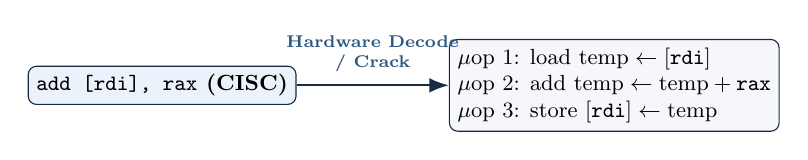
\begin{tikzpicture}[scale=0.88, every node/.style={transform shape}]
  \node[draw=navy, fill=lightblue, rounded corners=3pt, font=\small\bfseries, minimum width=3.5cm, minimum height=0.55cm] (x86) {\code{add [rdi], rax} (CISC)};
  
  \node[draw=navy, fill=softgray, rounded corners=3pt, font=\small, right=2.2cm of x86, align=left] (uops) {
    $\mu\text{op 1: } \text{load } \text{temp} \leftarrow [\code{rdi}]$ \\
    $\mu\text{op 2: } \text{add } \text{temp} \leftarrow \text{temp} + \code{rax}$ \\
    $\mu\text{op 3: } \text{store } [\code{rdi}] \leftarrow \text{temp}$
  };
  
  \draw[-{Latex[length=2.5mm]}, thick, navy] (x86) -- (uops) 
    node[midway, above=2pt, align=center, font=\scriptsize\bfseries, text=deepblue] {Hardware Decode \\ / Crack};
\end{tikzpicture}
\end{center}

\vfill
\begin{itemize}\setlength{\itemsep}{4pt}
  \item The execution core is an out-of-order engine processing RISC-like micro-operations ($\mu\text{ops}$).
  \item CISC-to-RISC translation occurs dynamically, incurring a front-end decode power overhead that RISC architectures natively bypass.
\end{itemize}
\end{frame}

% ============================================================
% Section 5 Divider
% ============================================================

\sectiondivider{SUMMARY \& ASSESSMENT}{Review and Self-Test Questions}

% ============================================================
% Slide 16: Comprehensive Summary
% ============================================================

\begin{frame}{Topic 2: Comprehensive Summary}

\begin{itemize}\setlength{\itemsep}{6pt}
  \item \key{Complexity Redistribution:} ISA design distributes work between compilers and hardware decoders.
  \item \key{CISC Trade-offs:} Prioritizes code density and low instruction count via variable-length instructions and register-memory operations, at the cost of front-end decode complexity.
  \item \key{RISC Trade-offs:} Prioritizes pipeline regularity, fixed 32-bit width, and explicit load/store architecture to achieve high clock frequency and low CPI.
  \item \key{Microarchitectural Convergence:} Modern x86 processors crack CISC instructions into internal RISC $\mu\text{ops}$, validating the core RISC execution model.
  \item \key{Evaluation Metrics:} True architectural efficiency is measured via the Iron Law ($T_{\text{CPU}} = \frac{\mathit{IC} \times \mathit{CPI}}{f_{\text{clk}}}$) and Performance-per-Watt.
\end{itemize}

\end{frame}

% ============================================================
% Slide 17: Self-Test Questions (Part 1)
% ============================================================

\begin{frame}{Self-Test Questions: ISA Principles \& Mechanics}

\begin{enumerate}\setlength{\itemsep}{6pt}
  \item \key{Load/Store Boundary:} Why does a strict load/store architecture simplify pipelined execution compared to an architecture permitting memory operands directly in ALU instructions?
  
  \vspace{0.2cm}
  \item \key{Parallel Decode Efficiency:} Why is an 8-wide instruction decoder significantly simpler and more power-efficient for a fixed 32-bit RISC ISA than for variable-length CISC?
  
  \vspace{0.2cm}
  \item \key{Micro-operation Translation:} When an x86 processor executes \code{add [rdi + 8], rax}, how does the front-end decoder functionally translate this instruction into internal $\mu\text{ops}$?
\end{enumerate}

\end{frame}

% ============================================================
% Slide 18: Self-Test Questions (Part 2)
% ============================================================

\begin{frame}{Self-Test Questions: Quantitative Analysis \& Power}

\begin{enumerate}\setlength{\itemsep}{6pt}
  \item \key{Iron Law Calculation:} A RISC core executes $1.5 \times 10^9$ instructions at $\text{CPI} = 1.1$ on a 3.0\,GHz CPU. A CISC core executes $1.1 \times 10^9$ instructions at $\text{CPI} = 1.6$ on a 3.2\,GHz CPU. Which finishes faster?
  
  \vspace{0.2cm}
  \item \key{Front-End Power Cost:} Why does instruction decoding consume a measurably higher percentage of core power in modern x86 processors than in modern AArch64 cores?
  
  \vspace{0.2cm}
  \item \key{Performance-per-Watt:} Why has Performance-per-Watt superseded raw clock frequency as the primary architectural design metric in modern computing?
\end{enumerate}

\end{frame}

% ============================================================
% Look Ahead to Topic 3 (Final Slide of Topic 2 Deck)
% ============================================================

\begin{frame}{Looking Ahead}

\begin{block}{Next Lecture Preview}
\key{Our Next Topic:} The Hardware/Software Interface \& AArch64 Programmer's Model
\end{block}

\vfill
\begin{itemize}\setlength{\itemsep}{7pt}
  \item \key{Architectural State:} Defining the precise software-visible hardware contract (registers, condition flags, stack pointer, and memory space).
  \item \key{AArch64 Register File:} Examining register naming conventions (\bits{x0}--\bits{x30} vs.\ \bits{w0}--\bits{w30}), the zero register (\bits{xzr}), and standard ABI calling conventions.
  \item \key{Instruction Mechanics:} Exploring foundational instruction classes, memory addressing modes, and control flow translation.
\end{itemize}
\vfill

\end{frame}

\end{document}